\phantomsection
\subsubsection*{Ֆունկցիաների համար հարցումներ}\label{subsubsec:functions}
\addcontentsline{toc}{subsubsection}{Ֆունկցիաների համար հարցումներ}

Այս հարցումները նույնպես բաժանվում են երկու խմբի՝
\begin{enumerate}
    \item ֆունկցիաների որոնման հարցումներ,
    \item ֆունկցիայի վերլուծության հարցումներ:
\end{enumerate}

Որոնման հարցումների միջոցով օգտագործողները կարող են որոնել և գտնել ֆունկցիաներն՝ օգտագործելով տարբեր ֆիլտրեր:
Նրանք կարող են որոնել ֆունկցիաներն ըստ՝
\begin{enumerate}
    \item անվանման,
    \item հայտարարող դասի,
    \item արգումենտների,
    \item կանչված ֆունկցիաների և այլն։
\end{enumerate}

Սա թույլ կտա օգտագործողներին արագ և թիրախավորված կերպով գտնել իրենց հետաքրքրող ֆունկցիաները:

Կոնկրետ ընտրված ֆունկցիայի համար օգտագործողը կարող է կատարել վերլուծության հարցումներ: Այդ հարցումների միջոցով հնարավոր
կլինի ստանալ տեղեկություններ՝
\begin{enumerate}
    \item տվյալ ֆունկցիան պարունակող դասերի մասին,
    \item հրահանգների մասին,
    \item այլ ֆունկցիաների հետ կապերի մասին և այլն։
\end{enumerate}

\begin{figure}[h]
    \centering
    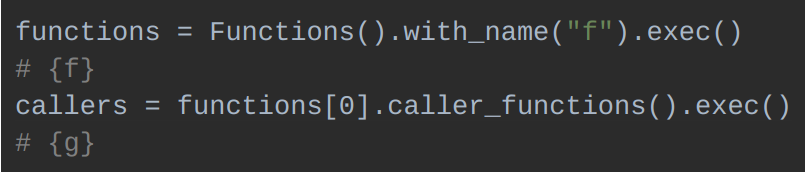
\includegraphics[width=0.6\textwidth]{pic14}
    \caption{Ֆունկցիաների համար հարցումների օրինակ}
    \label{fig:figure14}
\end{figure}

Այսպիսով, ֆունկցիաների համար նախատեսված որոնման և վերլուծության հարցումները թույլ կտան օգտագործողներին տեղեկանալ ֆունկցիաների
և դրանց փոխկապակցվածության մասին:
